\chapter{Theoretical background and materials}

\startcontents[chapters]
\printmyminitoc{
    
}



\section{Theoretical background}

\subsection{Topic modeling}

In NLP, topic modeling is a type of model that finds the overall topics that are shown in given documents, usually in the form of a corpus.

This method uses the statistic of the frequency of the words that appear in documents to identify the common between documents without knowing the predefined label and training data. For example in our case of a call center of an operator, a topic modeling algorithm could find whether the topic of documents are invoices, bills, telephones, or fiber based on their contents. Latent semantic analysis (LSA)\cite{deerwester-indexing-1990} latent Dirichlet analysis (LDA)\cite{944937} or Non-Negative Matrix Factorization (NMF)\cite{conf/nips/LeeS00} are some of the topic modeling methods that analyze large text files to categorize topics, provide valuable insights, and support better decision-making.

Topic modeling methods are also considered probabilistic topic models, which refer to statistical algorithms for discovering the latent semantic structures of an extensive text body. Nowadays, the amount of information that we receive each day is simply out of the ability of process of humans. This technique can help to organize and offer insights for us to understand the large amount of data that we encounter. From text-mining at first, topic modeling methods nowadays could also help to detect patterns in data such as genetic information, images, and networks. It also has applications in bioinformatics and computer vision.

\subsection{Word embedding}

In NLP, a word embedding is a representation of a word in the form of a vector in a vector space. The embedding is used in text analysis. Typically, the representation is a real-valued vector that encodes the meaning of the word in such a way that words that are closer in the vector space are expected to be similar in meaning. Word embeddings can be obtained using language modeling and feature learning techniques, where words or phrases from the vocabulary are mapped to vectors of real numbers.

Methods to generate this mapping include neural networks, dimensionality reduction on the word co-occurrence matrix, probabilistic models, explainable knowledge base method, and explicit representation in terms of the context in which words appear.

Word and phrase embeddings, when used as the input representation, have been proven to boost the performance in multiple NLP tasks such as syntactic parsing and sentiment analysis.

\subsection{Our way to find topics in a given corpus}

To reveal underlying common topics of a corpus, topic models have been shown to be an effective tool. Convention techniques like Latent Dirichlet Allocation (LDA)\cite{944937} or Non-Negative Matrix Factorization (NMF)\cite{conf/nips/LeeS00} describe corpus as a set of words and represent each document as a mixture of topics.

The big drawbacks of this method are they could lose the meaning and relation between words when it forms a bag-of-words, and it only uses the count of the number of words that appear in a document but does not account for the relationship and the context of words with each other inside a document.

For example, the word "bank", is the same in the river bank, and the bank is a place to store and borrow money if we apply Bag-of-Words\cite{bagofwords} and use LDA over it. However, if we apply a language model, the model could distinguish the differences between these 2 words "bank". They have the same representation but have different meanings due to different surrounding contexts.

We want to apply the advantage of language models to find the topics in a corpus.



\section{Materials}

\subsection{Tools}

\begin{figure}[H]
    \centering
    
\includegraphics[width=0.3\textwidth]{images/python.png}
    % \caption{Python}
    \label{fig:python_logo}
\end{figure}

This project was done by using Python. Python is one of the most popular programming languages in the field of data science, and for good reason. It offers numerous advantages that make it well-suited for data analysis, machine learning, and other data science tasks. Some of the key advantages of using Python in data science include:

\begin{itemize}
    \item \textbf{Rich Ecosystem of Libraries:} Python has a vast collection of libraries and frameworks specifically designed for data science tasks. Libraries like Numpy\cite{harris2020array}, pandas\cite{mckinney-proc-scipy-2010}, Matplotlib\cite{Hunter:2007}, Seaborn, and scikit-learn\cite{scikit-learn} provide powerful tools for data manipulation, analysis, visualization, and machine learning.
    \item \textbf{Versatility:}  Python is a general-purpose programming language, meaning that it's not limited to data science tasks. This versatility allows data scientists to integrate their work with other areas of development, creating end-to-end solutions. The extension of this project is not only about finding the topic of the dataset but also about building an end-to-end system for the usage of agents.
    \item \textbf{Jupyter Notebooks:}  Jupyter Notebooks\cite{Kluyver2016jupyter} provide an interactive and shareable environment for data analysis. They allow you to combine code, visualizations, and explanatory text in a single document, making it easy to document your work and share insights with others.
    \item \textbf{Data Visualization:}  Python offers several powerful visualization libraries, such as Matplotlib and Seaborn, that allow you to create informative and aesthetically pleasing graphs and charts to convey your findings effectively.
\end{itemize}

Besides common Python libraries that are used to process the data, for example, Pandas, Numpy, Scikit-learn, etc., it is necessary to use some of the famous libraries in the NLP field. Also, it is not recommended to do the preprocessing on a language model like BERT, but I do use Natural Language Toolkit (NLTK)\cite{bird2009natural} to do some light cleaning due to the original dataset containing a lot of noise. 

2 language models applied in this project are CamemBERT\cite{martin2020camembert} and MiniLMv2\cite{wang2021minilmv2} through the Sentence Transformer library. It helped to embed conversations and we represented both of them to find the best technique for our use case.

Scikit-learn is used to deploy clustering and dimension reduction techniques.

\subsection{Datasets}

The data that I use in this project is the transcribed call logs from the SFR customer care center database. In SFR, we use Apache Impala and Apache Hive to store information. However, to have permission to access such sensitive information, requires a special permit.

At first, I intended to use every call from June 2022, but it is proven that processing all of such huge data is considered too ambitious, with more than 7 billion words. My final dataset contains 100 million words from the first of June 2023 to the present.

The raw data table has a lot of information, but in the end, we only consider these columns.

\begin{table}[H]
\centering
\captionof{table}{Database description} \label{tab:description_database} 
\begin{tabular}{|lp{10cm}|lp{10cm}|}
\hline
\textbf{column name}  & \textbf{description}                                                                  \\ \hline
contact\_id           & ID of the conversation                                                                \\ \hline
transcript\_speaker   & 2 channels exist. Channel 1 is for our agent, and channel 2 is for the customer \\ \hline
transcript\_word      & Word of the transcript                                                                \\ \hline
transcript\_starttime & Time of each word when it is being spoken                                             \\ \hline
\end{tabular}
\end{table}

Each row in the table contains only one word, and the location is defined as the contact\_id, which is the id of the conversation and the transcript start time, with the beginning of the conversation as the second 0.

\begin{figure}[H]
    \centering
    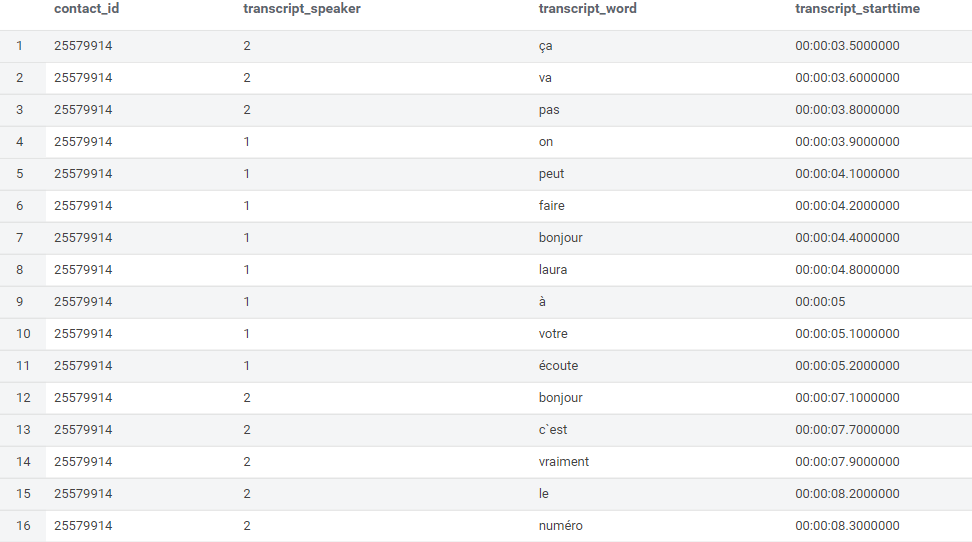
\includegraphics[width=1\textwidth]{images/db_example.png}
    \caption{Example of the format of the raw dataset}
    \label{fig:raw_dataset}
\end{figure}






